%:
\documentclass[9pt, oneside]{article}   	% use "amsart" instead of "article" for AMSLaTeX format
\usepackage{geometry}                		% See geometry.pdf to learn the layout options. There are lots.
\geometry{letterpaper}                   		% ... or a4paper or a5paper or ... 
%\geometry{landscape}                		% Activate for rotated page geometry
%\usepackage[parfill]{parskip}    		% Activate to begin paragraphs with an empty line rather than an indent
\usepackage{graphicx}				% Use pdf, png, jpg, or eps§ with pdflatex; use eps in DVI mode
								% TeX will automatically convert eps --> pdf in pdflatex		
\usepackage{amssymb}
\usepackage{diagbox}
\usepackage{amsmath}
\usepackage{amsthm}
\usepackage{enumerate}
\usepackage{tikz}
\usepackage{mathrsfs}
\usetikzlibrary{positioning}


\usetikzlibrary{arrows}
\theoremstyle{definition}
\newtheorem*{defn}{Definition}
\newtheorem*{prop}{Proposition}
\newtheorem*{eg}{Example}
\newtheorem*{thm}{Theorem}
\newtheorem*{corol}{Corollary}
\newtheorem{ex}{Exercise}[section]
{\theoremstyle{plain}
\newtheorem*{rmk}{Remark}
\newtheorem*{rmks}{Remarks}
\newtheorem*{lt}{Last time}
}
\newtheorem*{lem}{Lemma}
\usepackage{color}
\usepackage{CJK}
\title{Path to Efficient AGI}
\author{Xiyu Zhai}
\date{}							% Activate to display a given date or no date

\begin{document}
\maketitle
\tableofcontents

\section{Introduction}

This paper is the prelude of a series of papers that explore a new school of AI methodologies, which naturally incorporates with established AI methods like deep learning, and shall lead us towards \textbf{efficient} artificial general intelligence.

Here \textbf{efficiency} is the key because an inefficient AGI will take too long to appear or too expensive to be of important usage, although they could be helpful for entry level tasks. The meaning of efficiency is twofold:

\begin{enumerate}[(i)]
	\item Statistical efficiency. The ability to learn accurately from limited examples.
	\item Computational efficiency. The ability to perform computation in time and within resource boundary.
\end{enumerate}

Biological intelligence, especially that of human beings, border collies, huskies, etc, although being far more efficient than deep learning, is still far from perfection. We are already beaten by computer programs in terms of memorization or rule based computation. A prediction of this note is that, a near optimal AGI implementation over the architecture of CPUs and GPUs will be far superior than biological intelligence, let alone deep learning.

This paper is the blueprint of how to achieve efficient AGI, including

\begin{enumerate}[(i)]
	\item 
	\item 
	\item 
\end{enumerate}

It's going to be followed by

\begin{enumerate}[(i)]
	\item a paper on a new programming language called Husky, which satisfies the langauge requirments proposed;
	\item a paper on image classification based on ideas in section XX;
	\item a paper on image generation based on ideas in section XX;
\end{enumerate}

\section{Related Works}



\section{Theories Based on Turing Machines}

\subsection{Conventions}

For the matter of succinctness, we shall in this section restrict ourselves to Turing machine level when thinking of computation. This is of course far from reality, but it helps with illuminating the high level ideas.

By an $\textbf{NP}$ problem, we mean a decision problem together with the proof of that decision which can be verified in polynomial time.

Everything will be finite, i.e. representable in a Turing machine.

\subsection{NP Problems Arising from ML Problems}
\begin{center}
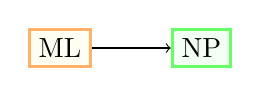
\begin{tikzpicture}[
roundnode/.style={rectangle, draw=green!60, fill=green!5, very thick, minimum size=4mm},
squarednode/.style={rectangle, draw=orange!60, fill=yellow!5, very thick, minimum size=4mm},
]
%Nodes
\node[squarednode]      (ml)                              {$\text{ML}$};
\node[roundnode]        (np)       		[right=of ml] {$\text{NP}$};

%Lines
\draw[->] (ml.east) -- (np.west);
\end{tikzpicture}
\end{center}

We begin with the well-known fundamental (non-unique) conversion of an ML problem into an NP problem.

An ML problem is about finding a function $f$ $\mathcal{X}\to \mathcal{Y}$ such that $\mathscr{L}(f):=\mathbb{E}_{(X,Y)\sim \mathcal{P}}l(f(X), Y)$ is small enough where $\mathcal{P}$ is an unknown distribution over $\mathcal{X}\times Y$ and $l:\mathcal{Y}\times \mathcal{Y} \to \mathbb{R}$ is a loss function, and we are given sampling from the unknown distribution $\mathcal{P}$ in a certain fashion (online or offline).

A model is a class $\mathcal{H}$ of functions from $\mathcal{X}$ to $\mathcal{Y}$ (called Hypothesis Space). We say the model is good if one of $f\in \mathcal{H}$ will make $\mathscr{L}(f)$ small enough.

Suppose that we're given enough data (the amount is still polynomial, which is possible if $\log \mathcal{H}$ is polynomial, which will be true if elements in $\mathcal{H}$ arer polynomially presentable), then $\widehat{\mathscr{L}}(f):=todo$ becomes a good approximation of $\mathscr{L}(f)$. Then whether the model is a good one becomes an NP problem, with the proof being the specific $f\in \mathcal{H}$ making $\widehat{\mathscr{L}}(f)$ small enough.

More generally, we could think of meta learning. Suppose we have a family of machine learning problems indexed by S, todo
\subsection{ML Problems Arising from NP Problems}
\begin{center}
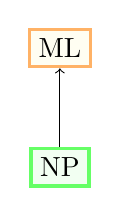
\begin{tikzpicture}[
roundnode/.style={rectangle, draw=green!60, fill=green!5, very thick, minimum size=4mm},
squarednode/.style={rectangle, draw=orange!60, fill=yellow!5, very thick, minimum size=4mm},
]
%Nodes
\node[roundnode]        (np)       		              {$\text{NP}$};
\node[squarednode]      (ml)           [above=of np]  {$\text{ML}$};

%Lines
\draw[->] (np.north) -- (ml.south);
\end{tikzpicture}
\end{center}

Given an NP problem, which consists of an input space $\mathcal{X}$, a certificate space $\mathcal{C}$, and a polytime verifier $v: \mathcal{X} \rightarrow \text{Bool}$, the goal is then to find an efficient implementation or approximation of $x\mapsto \exists_{c\in \mathcal{C}} v(x,c)$.

Let's start with some brute force method for find certificates, denoted by $c_{\text{brute}}(x): \mathcal{X} \to \mathcal{C}$.

Suppose that we are satisfied with the approximation $x\mapsto v(x,c_{\text{brute}}(x))$ and we only want to make it faster. We can collect a set of $x_i\in \mathcal{X}$, then build a dataset with $y_i=c_{brute}(x)$, then this becomes a machine learning problem.

(A more appropriate setup would be to make $c_{brute}(x)$ being a small finite set of certificates, and $v(x,c_{\text{brute}}(x))$ will become $\exists c\in c_{\text{brute}}(x), v(x, c)$)

Now in general we can't be satisfied with the simple approximation $x\mapsto v(x,c_{\text{brute}}(x))$, we can also use machine learning to make a better approximation.

One way is to divide and conquer. Factor $\mathcal{C}$ into a disjoint union $\sqcup_{i\in \mathcal{I}} \mathcal{C}_{i}$ indexed by a not necessarily small set $\mathcal{I}$. Then
\begin{equation}
	f_*(x)=\exists i\in \mathcal{I}, \exists c\in \mathcal{C}_i, v(x,c).
\end{equation}

Suppose that we have a brute force method $c_{\text{brute},i}$ for each $\mathcal{C}_i$. Define
\begin{equation}
	g: \mathcal{X}\times \mathcal{I} \rightarrow \text{Bool}, g(x, i) = v(x, c_{\text{brute},i}(x))
\end{equation}

Now $g$ is a function we can approximate with machine learning. Let the approximation we get be $\hat{g}$, then we can simplify the problem by searching within $\mathcal{I}$ of $s$

... RL is a special case.

\subsection{the Ladder of NP-ML Ascension}
``Good mathematicians see analogies. Great mathematicians see analogies between analogies.''

\hfill -- Stefan Banach, as in Banach Space


\begin{center}
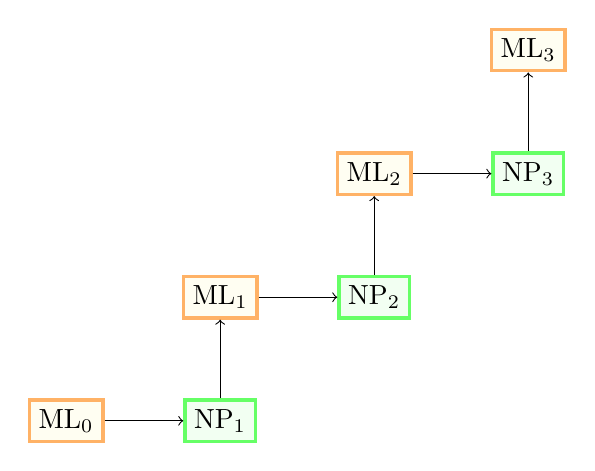
\begin{tikzpicture}[
roundnode/.style={rectangle, draw=green!60, fill=green!5, very thick, minimum size=4mm},
squarednode/.style={rectangle, draw=orange!60, fill=yellow!5, very thick, minimum size=4mm},
]
%Nodes
\node[squarednode]      (ml0)                              {$\text{ML}_0$};
\node[roundnode]        (np1)       		[right=of ml0] {$\text{NP}_1$};
\node[squarednode]      (ml1)       		[above=of np1] {$\text{ML}_1$};
\node[roundnode]        (np2)       		[right=of ml1] {$\text{NP}_2$};
\node[squarednode]      (ml2)       		[above=of np2] {$\text{ML}_2$};
\node[roundnode]        (np3)       		[right=of ml2] {$\text{NP}_3$};
\node[squarednode]      (ml3)       		[above=of np3] {$\text{ML}_3$};

%Lines
\draw[->] (ml0.east) -- (np1.west);
\draw[->] (np1.north) -- (ml1.south);
\draw[->] (ml1.east) -- (np2.west);
\draw[->] (np2.north) -- (ml2.south);
\draw[->] (ml2.east) -- (np3.west);
\draw[->] (np3.north) -- (ml3.south);
\end{tikzpicture}
\end{center}

The typical machine learnings algorithms including deep learning, typically doesn't go up beyond $NP_1$, that's why they can't achieve AGI and needs a lot of amount of data to fake AGI in restricted scenarios.

Todo: give many concrete examples. Many will come from programming and mathematics.

Todo: explain why it doesn't take much data to ascend.

\subsection{$NP_0$ Preceding $ML_0$: CV and NLP}


\section{Theories Based on Realistic Computation Models}



\section{Type System}

\subsection{Concept Level Types}


\subsection{System Level Types}

\subsection{Types for Machine Learning}

\section{Language Requirements}

\section{System}

\subsection{Database}

\subsection{Debugger}

\subsection{todo}

\section{Plans for Computer Vision}

\section{Plans for Natural Language Processing}

As claimed in previous sections, deep learning's success doesn't mean it's the optimal for natural language processing, but it will serve as a convenient tool for the development of a next generation far more superior tools.

Let's first conduct a worst scenario analysis. Suppose deep learning achieved AGI before us, and the AGI works amazingly well. Let's recall what makes symbolic AI methods like expert system fail: high development, maintenance, and debugging cost. But we can instruct deep learning AGI develop expert system and write out programs that parse English like parsing a programming language. It would take forever for humans, but for AGI, it would be trivial. The takeaway is, even if deep learning takes the holy grail, it won't keep it for very long as humans could then replace it a more rule-based AI with its help.

But this argument is not satisfying, due to the gloomy prospect of deep learning achieving AGI. Still there could be many practical approaches where we can leverage deep learning in its current form to build a more advanced form of AI, which I shall explain below.

\subsection{Stage 0: Domain Specific Verifiable Natural Language Processing}

We shall restrict ourselves to a very specific domain, relatively simple, so that we can easily build up a domain specific programming langauge to describe the tasks and also build efficient solvers for the task.
\begin{center}
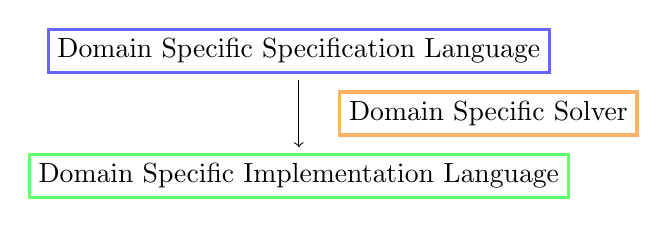
\begin{tikzpicture}[
squarednode1/.style={rectangle, draw=blue!60, fill=white!5, very thick, minimum size=4mm},
squarednode2/.style={rectangle, draw=green!60, fill=white!5, very thick, minimum size=4mm},
squarednode3/.style={rectangle, draw=orange!60, fill=white!5, very thick, minimum size=4mm},
]
%Nodes
\node[squarednode1]      (dssl)                              {Domain Specific Specification Language};
\node[squarednode2]      (dsil)              [below=of dssl]  {Domain Specific Implementation Language};

%Lines
\draw[->, shorten >=2pt, shorten <=2pt] (dssl.south) -- (dsil.north) node[squarednode3, midway, right, xshift=5mm] {Domain Specific Solver};
\end{tikzpicture}
\end{center}

\begin{eg}
	[Mathematica]
\end{eg}

\begin{eg}
	[Html, Css] Html and Css are not specification languages, they are implementation languages.
\end{eg}

Let's compare the pros and cons with ChatGPT

Here's a nice summary in table \ref{comparison} written by the very ChatGPT itself.

\begin{table}[ht]
\label{comparison}
\centering
\small % reduce font size
\begin{tabular}{|l|p{6cm}|p{6cm}|}
\hline
 & \textbf{ChatGPT} & \textbf{DSLs} \\
\hline
\textbf{Pros} & 
Flexibility: ChatGPT can be used for a wide variety of NLP tasks, including text generation, question answering, summarization, and more.
&
Increased productivity: DSLs are designed to be easy to use and understand within a specific domain, which can increase developer productivity. \\
\cline{2-3}
& 
Ease of use: ChatGPT can be accessed through simple API calls or integrated into other applications and platforms.
&
Enhanced control: A DSL provides more fine-grained control over a specific problem within a domain, allowing developers to tailor their solutions to specific requirements. \\
\cline{2-3}
& 
Low development time: Implementing a ChatGPT-based solution typically requires less development time than creating a custom DSL.
&
Improved maintainability: DSLs can make code more readable and maintainable within a specific domain, as they typically use domain-specific terminology and concepts. \\
\cline{2-3}
& 
Multilingual support: ChatGPT can generate text in multiple languages.
&
 \\
\hline
\textbf{Cons} & 
Limited control: ChatGPT generates text based on its training data and can sometimes produce unexpected or incorrect output.
&
Higher development time: Developing a custom DSL can require a significant amount of time and effort. \\
\cline{2-3}
& 
Lack of transparency: It can be difficult to understand why ChatGPT generates a particular piece of text, making it hard to debug or fine-tune.
&
Limited flexibility: A DSL is designed to solve a specific problem within a specific domain, so it may not be suitable for other tasks or domains. \\
\cline{2-3}
& 
Dependence on data quality: The quality of ChatGPT's output is heavily dependent on the quality and diversity of its training data.
&
Steep learning curve: Developers may need to learn a new syntax and programming paradigm in order to use a DSL effectively. \\
\hline
\end{tabular}
\caption{Comparison of ChatGPT and DSLs}
\label{tab:chatgpt-dsls}
\end{table}

I'm sorry that I have to copy because my hands are not in 100\% health.

\clearpage

We could have the best of both worlds by combining dsls with deep learning like this:
\begin{center}
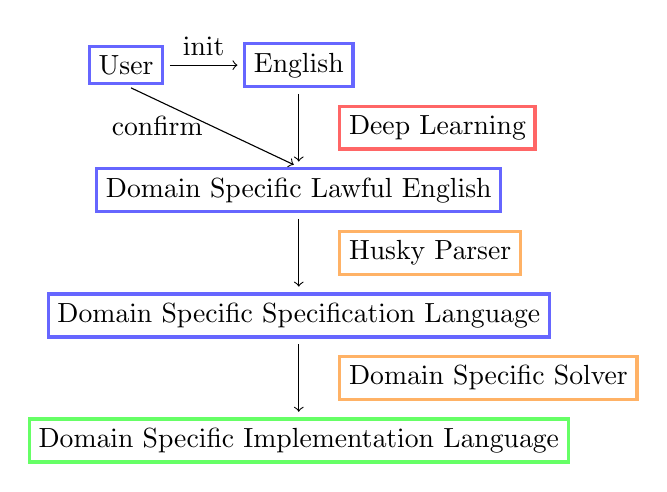
\begin{tikzpicture}[
squarednode1/.style={rectangle, draw=blue!60, fill=white!5, very thick, minimum size=4mm},
squarednode2/.style={rectangle, draw=green!60, fill=white!5, very thick, minimum size=4mm},
squarednode3/.style={rectangle, draw=orange!60, fill=white!5, very thick, minimum size=4mm},
squarednode4/.style={rectangle, draw=red!60, fill=white!5, very thick, minimum size=4mm},
]
%Nodes
\node[squarednode1]              (user)                              {User};
\node[squarednode1]      (e)             [right=of user]   {English};
\node[squarednode1]      (dsle)             [below=of e]   {Domain Specific Lawful English};
\node[squarednode1]      (dssl)             [below=of dsle]    {Domain Specific Specification Language};
\node[squarednode2]      (dsil)              [below=of dssl]  {Domain Specific Implementation Language};

%Lines
\draw[->, shorten >=2pt, shorten <=2pt] (user.east) -- (e.west) node[midway, above] {init};
\draw[->, shorten >=2pt, shorten <=2pt] (user.south) -- (dsle.north) node[midway, left] {confirm};
\draw[->, shorten >=2pt, shorten <=2pt] (e.south) -- (dsle.north) node[squarednode4, midway, right, xshift=5mm] {Deep Learning};
\draw[->, shorten >=2pt, shorten <=2pt] (dsle.south) -- (dssl.north) node[squarednode3, midway, right, xshift=5mm] {Husky Parser};
\draw[->, shorten >=2pt, shorten <=2pt] (dssl.south) -- (dsil.north) node[squarednode3, midway, right, xshift=5mm] {Domain Specific Solver};
\end{tikzpicture}
\end{center}

First, we create a subset of English called Domain Specific Lawful English such as
\begin{enumerate}[(i)]
	\item it's grammarly and semantically rigorous, so that parsing in Husky code is feasible (although it might be too difficult for traditional languages like C++/Rust/Python/Haskell)
	\item it's expressive enough for the domain and can be faithfully translated into the Domain Specific Specification Language
	\item easily understood by users
\end{enumerate}

Second, we collect data and train a deep neural network that can translate arbitrary English into the subset.

When user initializes a dialogue using arbitrary English, it's translated into Domain Specific Lawful English, which is checked by the Husky Parser and also confirmed by the user that the translation is correct.

Then the Domain Specific Lawful English is translated by the Husky Parser into Domain Specific Specification Language so that it's acceptable by the solver.

Obviously, this setup will have the advantages of both worlds.

The details will be covered in the followup papers.

\subsection{Stage 1: Universal Lawful English}

Todo

\subsection{Stage 2: Minimizing Usage of Deep Learning}

Todo

\subsection{Stage 3: Learning Augmented Verifiable Solver}

Todo

\subsection{Stage 4: Generating Human Readable Explanations}

Todo

\end{document}